%% This is an example first chapter.  You should put chapter/appendix that you
%% write into a separate file, and add a line \include{yourfilename} to
%% main.tex, where `yourfilename.tex' is the name of the chapter/appendix file.
%% You can process specific files by typing their names in at the
%% \files=
%% prompt when you run the file main.tex through LaTeX.
\section{Disk Graph studies}

\subsection{Stabbing disks}

Definition of stabbing.

Stabbing geometric structures.\cite{schlipf2013stabbing}

\subsection{Thin Strip Graphs}

$c$-strip graphs are unit disk graphs such that the centers of the disks are delimited on the area $\{(x,y) : -\infty < x < \infty, 0 < y \leq c\}$ and its class noted SG($c$). We can say that SG(0) = UIG and SG($\infty$) = UDG. \cite{hayashiThinStripGraphs2017}

\begin{defn}
  Thin strip graphs are defined as TSG $= \bigcap_{c > 0}$ SG($c$).
\end{defn}

\begin{remark}
  SG($0$) $\neq$ TSG. This can be seen
\end{remark}

\begin{figure}
\centering
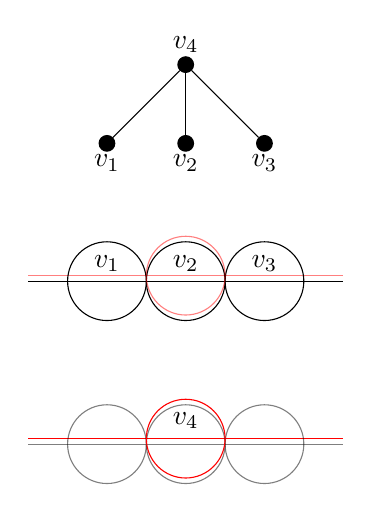
\begin{tikzpicture}
\draw (-2,0) -- (2,0);
\draw[red ,opacity = 0.5] (-2,0.07) -- (2,0.07);
\draw  (-1,0) circle [radius=0.5];
\draw[color=black] (-1,0.2265) node {$v_1$};
\draw  (0,0) circle [radius=0.5];
\draw[color=black] (0,0.2265) node {$v_2$};
\draw  (1,0) circle [radius=0.5];
\draw[color=black] (1,0.2265) node {$v_3$};

\draw[red, opacity = 0.5] (0,0.07) circle [radius=0.5];

\draw[opacity = 0.5] (-2,-2.07) -- (2,-2.07);
\draw[red] (-2,-2) -- (2,-2);
\draw[opacity = 0.5]  (0,-2.07) circle [radius=0.5];
\draw[opacity = 0.5]  (1,-2.07) circle [radius=0.5];
\draw[opacity = 0.5]  (-1,-2.07) circle [radius=0.5];
\draw[red] (0,-2) circle [radius=0.5];
\draw[color=black] (0,-1.765) node {$v_4$};

\node[draw,circle,inner sep=2pt,fill,label distance=1cm] (v1) at (0,2.75) {};
\draw[color=black] (0,3) node {$v_4$};
\node[draw,circle,inner sep=2pt,fill,label distance=1cm] (v3) at (0,1.75) {};
\draw[color=black] (0,1.5) node {$v_2$};
\node[draw,circle,inner sep=2pt,fill,label distance=1cm] (v2) at (-1,1.75) {};
\draw[color=black] (1,1.5) node {$v_3$};
\node[draw,circle,inner sep=2pt,fill,label distance=1cm] (v4) at (1,1.75) {};
\draw[color=black] (-1,1.5) node {$v_1$};
\draw  (v1) edge (v2);
\draw  (v1) edge (v3);
\draw  (v1) edge (v4);
\end{tikzpicture}
\end{figure}

$K_{1,3}$ in TSG, which is not possible for UIG.

MUIG $\subsetneq$ TSG.\\


Denote that there's not constant $t$ such that SG($t$) = TSG.\\

Unfettered unit interval graphs = UUIG\\

MUIG $\subsetneq$ TSG $\subsetneq$ UUIG

\begin{defn}
  Find forbidden induced graphs for TSG.
\end{defn}
